\documentclass[11pt]{article}
\usepackage[utf8]{inputenc}
\usepackage{amsmath}
\usepackage{amsfonts}
\usepackage{amssymb}
\usepackage{geometry}
\usepackage{enumitem}
\usepackage{graphicx}
\usepackage{tikz}
\usepackage{pgfplots}
\usepackage{amsthm}
\usepackage{mathtools}

\geometry{margin=1in}

\theoremstyle{definition}
\newtheorem{definition}{Definition}[section]
\newtheorem{theorem}{Theorem}[section]
\newtheorem{lemma}{Lemma}[section]
\newtheorem{corollary}{Corollary}[section]
\newtheorem{example}{Example}[section]
\newtheorem{proposition}{Proposition}[section]

\title{Statistics Summary}
\author{Mathematical Notes}
\date{\today}

\begin{document}

\maketitle

\tableofcontents
\newpage

\section{Descriptive Statistics}

\subsection{Measures of Central Tendency}
\begin{definition}
For a sample $x_1, x_2, \ldots, x_n$:
\begin{itemize}
    \item \textbf{Mean}: $\bar{x} = \frac{1}{n}\sum_{i=1}^n x_i$
    \item \textbf{Median}: Middle value when data is ordered
    \item \textbf{Mode}: Most frequently occurring value
\end{itemize}
\end{definition}

\subsection{Measures of Dispersion}
\begin{definition}
\begin{itemize}
    \item \textbf{Variance}: $s^2 = \frac{1}{n-1}\sum_{i=1}^n (x_i - \bar{x})^2$
    \item \textbf{Standard Deviation}: $s = \sqrt{s^2}$
    \item \textbf{Range}: $\max(x_i) - \min(x_i)$
    \item \textbf{Interquartile Range}: $Q_3 - Q_1$
\end{itemize}
\end{definition}

\section{Parameter Estimation}

\subsection{Point Estimation}
\begin{definition}
A \textbf{point estimator} $\hat{\theta}$ is a statistic used to estimate a population parameter $\theta$.
\end{definition}

\subsection{Properties of Estimators}
\begin{definition}
An estimator $\hat{\theta}$ is:
\begin{itemize}
    \item \textbf{Unbiased} if $E[\hat{\theta}] = \theta$
    \item \textbf{Consistent} if $\hat{\theta} \xrightarrow{p} \theta$ as $n \to \infty$
    \item \textbf{Efficient} if it has minimum variance among unbiased estimators
\end{itemize}
\end{definition}

\subsection{Maximum Likelihood Estimation}
\begin{definition}
The \textbf{maximum likelihood estimator} (MLE) is the value of $\theta$ that maximizes the likelihood function $L(\theta) = \prod_{i=1}^n f(x_i|\theta)$.
\end{definition}

\subsection{Method of Moments}
\begin{definition}
The \textbf{method of moments} estimator equates sample moments to population moments:
$$\frac{1}{n}\sum_{i=1}^n X_i^k = E[X^k]$$
\end{definition}

\section{Confidence Intervals}

\subsection{Definition}
\begin{definition}
A \textbf{confidence interval} for parameter $\theta$ is an interval $[L, U]$ such that $P(L \leq \theta \leq U) = 1 - \alpha$.
\end{definition}

\subsection{Common Confidence Intervals}

\subsubsection{Normal Mean (Known Variance)}
For $X \sim \mathcal{N}(\mu, \sigma^2)$ with known $\sigma^2$:
$$\bar{X} \pm z_{\alpha/2} \frac{\sigma}{\sqrt{n}}$$

\subsubsection{Normal Mean (Unknown Variance)}
For $X \sim \mathcal{N}(\mu, \sigma^2)$ with unknown $\sigma^2$:
$$\bar{X} \pm t_{\alpha/2,n-1} \frac{s}{\sqrt{n}}$$

\subsubsection{Proportion}
For binomial proportion $p$:
$$\hat{p} \pm z_{\alpha/2} \sqrt{\frac{\hat{p}(1-\hat{p})}{n}}$$

% Illustration of confidence intervals
\begin{figure}[h]
\centering
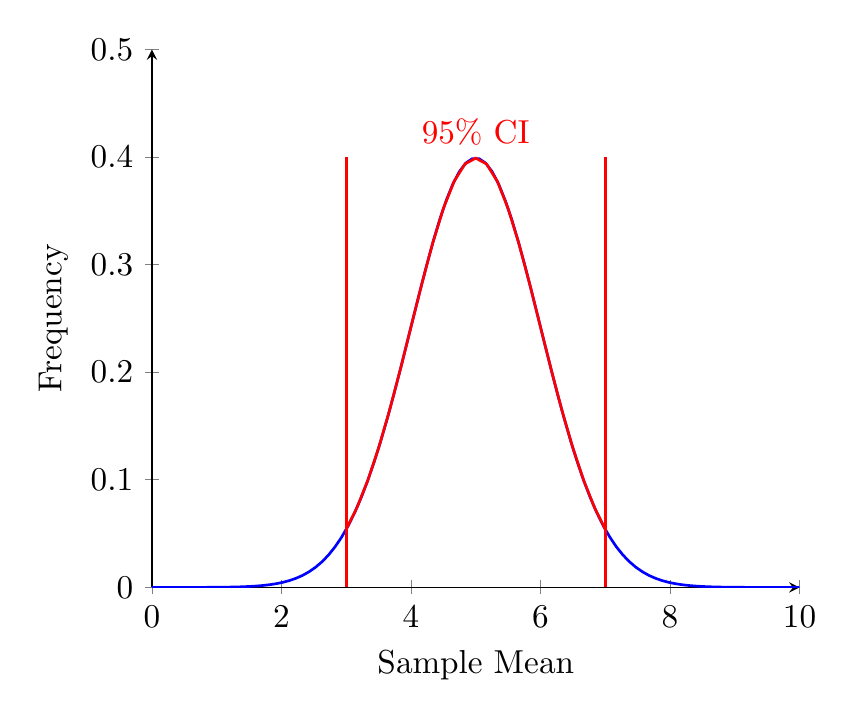
\begin{tikzpicture}[scale=1.2]
    \begin{axis}[
        axis lines = left,
        xlabel = Sample Mean,
        ylabel = Frequency,
        xmin=0, xmax=10,
        ymin=0, ymax=0.5,
    ]
    
    % Normal distribution
    \addplot[blue, thick, domain=0:10, samples=100] {exp(-(x-5)^2/2)/sqrt(2*pi)};
    
    % Confidence interval
    \addplot[red, thick, domain=3:7] {exp(-(x-5)^2/2)/sqrt(2*pi)};
    \addplot[red, thick] coordinates {(3,0) (3,0.4)};
    \addplot[red, thick] coordinates {(7,0) (7,0.4)};
    
    \node[red, above] at (5,0.4) {95\% CI};
    
    \end{axis}
\end{tikzpicture}
\caption{Confidence interval for normal distribution}
\end{figure}

\section{Hypothesis Testing}

\subsection{Basic Concepts}
\begin{definition}
A \textbf{hypothesis test} is a procedure for deciding between two competing hypotheses:
\begin{itemize}
    \item $H_0$: Null hypothesis
    \item $H_1$: Alternative hypothesis
\end{itemize}
\end{definition}

\subsection{Types of Errors}
\begin{definition}
\begin{itemize}
    \item \textbf{Type I Error}: Reject $H_0$ when it's true (probability $\alpha$)
    \item \textbf{Type II Error}: Fail to reject $H_0$ when it's false (probability $\beta$)
    \item \textbf{Power}: $1 - \beta = P(\text{reject } H_0 | H_1 \text{ true})$
\end{itemize}
\end{definition}

\subsection{Test Statistics}

\subsubsection{Z-Test}
For testing mean with known variance:
$$Z = \frac{\bar{X} - \mu_0}{\sigma/\sqrt{n}} \sim \mathcal{N}(0,1)$$

\subsubsection{t-Test}
For testing mean with unknown variance:
$$t = \frac{\bar{X} - \mu_0}{s/\sqrt{n}} \sim t_{n-1}$$

\subsubsection{Chi-Square Test}
For testing variance:
$$\chi^2 = \frac{(n-1)s^2}{\sigma_0^2} \sim \chi^2_{n-1}$$

\subsection{p-Values}
\begin{definition}
The \textbf{p-value} is the probability of observing a test statistic as extreme or more extreme than the observed value, assuming $H_0$ is true.
\end{definition}

\section{Regression Analysis}

\subsection{Simple Linear Regression}
\begin{definition}
The simple linear regression model is:
$$Y_i = \beta_0 + \beta_1 X_i + \epsilon_i$$
where $\epsilon_i \sim \mathcal{N}(0, \sigma^2)$.
\end{definition}

\subsection{Least Squares Estimation}
The least squares estimators are:
$$\hat{\beta_1} = \frac{\sum_{i=1}^n (X_i - \bar{X})(Y_i - \bar{Y})}{\sum_{i=1}^n (X_i - \bar{X})^2}$$
$$\hat{\beta_0} = \bar{Y} - \hat{\beta_1}\bar{X}$$

\subsection{Coefficient of Determination}
\begin{definition}
The \textbf{coefficient of determination} is:
$$R^2 = \frac{\text{SSR}}{\text{SST}} = 1 - \frac{\text{SSE}}{\text{SST}}$$
where SSR is sum of squares due to regression, SSE is sum of squared errors, and SST is total sum of squares.
\end{definition}

% Illustration of regression
\begin{figure}[h]
\centering
\begin{tikzpicture}[scale=1.2]
    \begin{axis}[
        axis lines = left,
        xlabel = $X$,
        ylabel = $Y$,
        xmin=0, xmax=10,
        ymin=0, ymax=10,
    ]
    
    % Data points
    \addplot[blue, only marks, mark=*] coordinates {
        (1,2) (2,3.5) (3,4) (4,5.5) (5,6) (6,7.5) (7,8) (8,9) (9,9.5)
    };
    
    % Regression line
    \addplot[red, thick, domain=0:10] {0.9*x + 1.2};
    
    \node[red, above] at (5,6) {$\hat{Y} = 0.9X + 1.2$};
    
    \end{axis}
\end{tikzpicture}
\caption{Simple linear regression}
\end{figure}

\subsection{Multiple Linear Regression}
\begin{definition}
The multiple linear regression model is:
$$Y_i = \beta_0 + \beta_1 X_{i1} + \beta_2 X_{i2} + \cdots + \beta_p X_{ip} + \epsilon_i$$
\end{definition}

\subsection{ANOVA}
\begin{definition}
\textbf{Analysis of Variance} (ANOVA) tests whether the means of several groups are equal:
$$F = \frac{\text{MSB}}{\text{MSW}} \sim F_{k-1, n-k}$$
where MSB is mean square between groups and MSW is mean square within groups.
\end{definition}

\section{Bayesian Inference}

\subsection{Bayes' Theorem}
\begin{theorem}
$$P(\theta|data) = \frac{P(data|\theta)P(\theta)}{P(data)} = \frac{L(\theta)\pi(\theta)}{\int L(\theta)\pi(\theta)d\theta}$$
where $\pi(\theta)$ is the prior distribution and $P(\theta|data)$ is the posterior distribution.
\end{theorem}

\subsection{Prior Distributions}
\begin{definition}
Common conjugate priors:
\begin{itemize}
    \item Normal-Normal: $X|\mu \sim \mathcal{N}(\mu, \sigma^2)$, $\mu \sim \mathcal{N}(\mu_0, \tau^2)$
    \item Beta-Binomial: $X|p \sim \text{Binomial}(n,p)$, $p \sim \text{Beta}(\alpha, \beta)$
    \item Gamma-Poisson: $X|\lambda \sim \text{Poisson}(\lambda)$, $\lambda \sim \text{Gamma}(\alpha, \beta)$
\end{itemize}
\end{definition}

\subsection{Bayesian Estimation}
\begin{definition}
Bayesian point estimators:
\begin{itemize}
    \item \textbf{Posterior Mean}: $E[\theta|data]$
    \item \textbf{Posterior Median}: Median of posterior distribution
    \item \textbf{Maximum A Posteriori (MAP)}: Mode of posterior distribution
\end{itemize}
\end{definition}

\section{Nonparametric Methods}

\subsection{Goodness of Fit Tests}

\subsubsection{Kolmogorov-Smirnov Test}
\begin{definition}
Tests whether a sample comes from a specified distribution:
$$D_n = \sup_x |F_n(x) - F_0(x)|$$
where $F_n$ is the empirical CDF and $F_0$ is the hypothesized CDF.
\end{definition}

\subsubsection{Chi-Square Goodness of Fit}
\begin{definition}
$$\chi^2 = \sum_{i=1}^k \frac{(O_i - E_i)^2}{E_i} \sim \chi^2_{k-1}$$
where $O_i$ are observed frequencies and $E_i$ are expected frequencies.
\end{definition}

\subsection{Rank Tests}

\subsubsection{Wilcoxon Rank-Sum Test}
Tests whether two independent samples come from the same distribution.

\subsubsection{Mann-Whitney U Test}
Nonparametric alternative to the two-sample t-test.

\section{Time Series Analysis}

\subsection{Stationarity}
\begin{definition}
A time series is \textbf{stationary} if:
\begin{itemize}
    \item $E[X_t] = \mu$ (constant mean)
    \item $\text{Var}(X_t) = \sigma^2$ (constant variance)
    \item $\text{Cov}(X_t, X_{t+k}) = \gamma(k)$ (covariance depends only on lag)
\end{itemize}
\end{definition}

\subsection{ARIMA Models}
\begin{definition}
An \textbf{ARIMA}(p,d,q) model is:
$$\phi(B)(1-B)^d X_t = \theta(B)\epsilon_t$$
where $B$ is the backshift operator, $\phi(B)$ is the AR polynomial, and $\theta(B)$ is the MA polynomial.
\end{definition}

\section{Design of Experiments}

\subsection{Randomized Controlled Trials}
\begin{definition}
A \textbf{randomized controlled trial} randomly assigns subjects to treatment and control groups to minimize bias.
\end{definition}

\subsection{Factorial Designs}
\begin{definition}
A \textbf{factorial design} studies the effect of multiple factors simultaneously:
$$Y_{ijk} = \mu + \alpha_i + \beta_j + (\alpha\beta)_{ij} + \epsilon_{ijk}$$
\end{definition}

\subsection{Blocking}
\begin{definition}
\textbf{Blocking} groups similar experimental units together to reduce variability and increase precision.
\end{definition}

\section{Multivariate Statistics}

\subsection{Multivariate Normal Distribution}
\begin{definition}
A random vector $\mathbf{X} = (X_1, \ldots, X_p)^T$ has a multivariate normal distribution if:
$$f(\mathbf{x}) = \frac{1}{(2\pi)^{p/2}|\boldsymbol{\Sigma}|^{1/2}} \exp\left(-\frac{1}{2}(\mathbf{x}-\boldsymbol{\mu})^T\boldsymbol{\Sigma}^{-1}(\mathbf{x}-\boldsymbol{\mu})\right)$$
\end{definition}

\subsection{Principal Component Analysis}
\begin{definition}
\textbf{Principal Component Analysis} (PCA) finds linear combinations of variables that explain maximum variance:
$$\mathbf{Y} = \mathbf{A}\mathbf{X}$$
where $\mathbf{A}$ is chosen to maximize variance of $\mathbf{Y}$.
\end{definition}

\subsection{Canonical Correlation}
\begin{definition}
\textbf{Canonical correlation} finds linear combinations of two sets of variables that are maximally correlated.
\end{definition}

\section{Applications}

\subsection{Clinical Trials}
Statistics is essential for:
\begin{itemize}
    \item Sample size determination
    \item Randomization procedures
    \item Interim analyses
    \item Safety monitoring
\end{itemize}

\subsection{Quality Control}
Applications include:
\begin{itemize}
    \item Control charts
    \item Process capability analysis
    \item Design of experiments
    \item Reliability analysis
\end{itemize}

\subsection{Survey Sampling}
Used in:
\begin{itemize}
    \item Population estimation
    \item Stratified sampling
    \item Cluster sampling
    \item Nonresponse adjustment
\end{itemize}

\section{Important Theorems}

\subsection{Central Limit Theorem}
\begin{theorem}
If $X_1, X_2, \ldots$ are i.i.d. with mean $\mu$ and variance $\sigma^2$, then:
$$\frac{\sqrt{n}(\bar{X}_n - \mu)}{\sigma} \xrightarrow{d} \mathcal{N}(0,1)$$
\end{theorem}

\subsection{Slutsky's Theorem}
\begin{theorem}
If $X_n \xrightarrow{d} X$ and $Y_n \xrightarrow{p} c$, then:
\begin{itemize}
    \item $X_n + Y_n \xrightarrow{d} X + c$
    \item $X_n Y_n \xrightarrow{d} cX$
    \item $X_n / Y_n \xrightarrow{d} X / c$ (if $c \neq 0$)
\end{itemize}
\end{theorem}

\subsection{Delta Method}
\begin{theorem}
If $\sqrt{n}(\hat{\theta}_n - \theta) \xrightarrow{d} \mathcal{N}(0, \sigma^2)$ and $g$ is differentiable at $\theta$, then:
$$\sqrt{n}(g(\hat{\theta}_n) - g(\theta)) \xrightarrow{d} \mathcal{N}(0, [g'(\theta)]^2 \sigma^2)$$
\end{theorem}

\end{document}
